\documentclass[letterpaper,11pt]{article}
\usepackage[spanish]{babel}
\usepackage[utf8]{inputenc}
\usepackage{graphicx}
\usepackage{amsfonts,amsmath,amssymb,float, amsthm,mathrsfs}  
\usepackage[right=4.5cm,left=2cm,top=3cm,bottom=3cm,headsep= 0.7cm,footskip=0.5cm]{geometry}
\usepackage{enumerate}
\usepackage{wrapfig} 
\usepackage[rflt]{floatflt} 
\usepackage{framed}
%\usepackage[most]{tcolorbox}
\usepackage[dvipsnames]{xcolor}
\colorlet{shadecolor}{green!20}
\setlength\FrameSep{0.5ex}
\usepackage{thmtools}
\usepackage{esint}
\usepackage{cancel}
\usepackage{listings} 
\usepackage{pstricks, caption}
\usepackage[colorlinks]{hyperref}
\usepackage{csquotes}
\usepackage{fullpage}
\usepackage{enumitem}
\usepackage{etoolbox}
\usepackage{tikz}
\usepackage{tikz-3dplot}
\tdplotsetmaincoords{80}{70}
\usetikzlibrary{decorations.markings}
\usetikzlibrary{arrows,babel}
\usepackage[font=small]{caption}
\usepackage{scalerel} %\scaleto{text}{size}
\usepackage{subcaption}
\usepackage{fancyhdr}
\usepackage{comment}
\usepackage{marginnote}
\usepackage{tensor}
\usepackage{cleveref}
\newcommand{\dbar}{\mathchar'26\mkern-12mu d}
\renewcommand*{\marginnotevadjust}{-0.1cm}
\renewcommand*{\marginfont}{\footnotesize}
\setlength{\headheight}{15pt}
\addtolength{\topmargin}{-14.49998pt}
\setlength{\headsep}{15pt}
\setlength{\footskip}{14.49998pt}
\decimalpoint
\newcommand{\grad}{^\circ}
\newlength{\drop}
\DeclareMathOperator{\sign}{sgn}
\DeclareMathOperator{\Log}{Log}
\providecommand{\norm}[1]{\lVert#1\rVert}

\let\cancelorigcolor\CancelColor% Just for conveniency...

\newcommand{\CancelTo}[3][]{%
  \ifblank{#1}{}{%
    \renewcommand{\CancelColor}{#1}%
  }
  \cancelto{#2}{#3}% 
}


\begin{document}

\pagestyle{plain}

\begin{flushleft}\vspace{-2cm}
Departamento de Física \\
Facultad de Cs. Físicas y Matemáticas\\
Universidad de Concepción
\end{flushleft}

\begin{flushright}\vspace{-1.5cm}
\textbf{Tópicos en Relatividad General} 
\end{flushright}



\rule{\linewidth}{0.1mm}

\begin{center}
\textbf{\LARGE Semana 13}
\end{center}

\begin{flushleft}
\textbf{Nombre:} Alejandro Saavedra San Martín. \\
\textbf{Profesor:} Guillermo Rubilar Alegría.
\end{flushleft}

\section{Campos gravitacionales débiles y ondas gravitacionales}

\subsection{Generación de ondas gravitacionales}

Recordemos que, en el gauge de Lorenz, las ecuaciones de Einstein linealizadas asumen la forma
\begin{equation}
\square \bar{h}_{\mu\nu} = - \frac{16\pi G}{c^4} T_{\mu\nu}^{(0)}, \qquad \partial^{\nu} \bar{h}_{\mu\nu} = 0.
\end{equation}

Las soluciones particulares corresponden a campos retardados asintóticamente nulos de la forma
\begin{equation}
\bar{h}_{\mu\nu}(\vec{x},t) = -  \frac{4G}{c^4} \int \frac{T_{\mu\nu}^{(0)}(\vec{x}\,', t_{\text{ret}})}{|\vec{x} - \vec{x}\,'|} d^3x', \label{eq:sol-GW}
\end{equation}
donde $t_{\text{ret}} =  t - |\vec{x} - \vec{x}\,'|/c$ es el \textit{tiempo retardado}.

Siguiendo el caso de ondas electromagnéticas, consideremos distancias muy grandes (en la zona lejana o zona de radiación, $r \gg \lambda$) y para fuentes pequeñas (de tamaño $L \ll \lambda$), ver figura \ref{fig:emision-GW-1}. Si $|\vec{x}| = r$, entonces para $\vec{x}\,'/r \ll 1$, tenemos que
\begin{align}
|\vec{x} - \vec{x}\,'| &= \left|r \hat{r} - \vec{x}\,'\right| \nonumber \\
&= r \left|\hat{r} - \frac{\vec{x}\,'}{r}\right| \nonumber \\
&= r \sqrt{\left( \hat{r} - \frac{\vec{x}\,'}{r}\right)\left( \hat{r} - \frac{\vec{x}\,'}{r}\right)}\nonumber \\
&= r \sqrt{1 - 2 \frac{\vec{x}\,'\cdot \hat{r}}{r} + \mathcal{O}(r^{-2})} \nonumber \\
&= r \left(1 - \frac{\vec{x}\,'\cdot \hat{r}}{r} + \mathcal{O}(r^{-2}) \right) \nonumber \\
&= r - \vec{x}\,' \cdot  \hat{r} + \mathcal{O}(r^{-1}).
\end{align}

Luego, tomando el recíproco, obtenemos
\begin{align}
\frac{1}{|\vec{x} - \vec{x}\,'|} &\approx \frac{1}{r - \vec{x}\,' \cdot  \hat{r}} \nonumber \\
&= \frac{1}{r} \frac{1}{1 - \frac{\vec{x}\,' \cdot  \hat{r}}{r}}  \nonumber \\
&= \frac{1}{r} \left(1 + \frac{\hat{r}\cdot \vec{x}\,'}{r} + \mathcal{O}(r^{-2}) \right) \nonumber \\
&= \frac{1}{r} + \mathcal{O}(r^{-2}).
\end{align}

Reemplazando en la expresión del tiempo retardado, encontramos que, bajo estas aproximaciones,
\begin{equation}
t_{\text{ret}} = t - \frac{|\vec{x} - \vec{x}\,'|}{c} = t - \frac{r}{c} + \frac{\vec{x}\,'\cdot \hat{r}}{c} + \mathcal{O}(r^{-1}).
\end{equation}

Para calcular la perturbación de la métrica incluyendo términos hasta orden $1/r$ es suficiente expandir $T_{\mu\nu}^{(0)}(\vec{x}\,',t_{\text{ret}})$ a orden cero en potencias de $1/r$, es decir,
\begin{equation}
T_{\mu\nu}^{(0)}(\vec{x}\,',t_{\text{ret}}) = T_{\mu\nu}^{(0)}\left(\vec{x}\,', t - \frac{r}{c} + \frac{\vec{x}\,'\cdot\hat{r}}{c}\right) + \mathcal{O}(r^{-1}),
\end{equation}
de modo que 
\begin{equation}
\frac{T_{\mu\nu}^{(0)}(\vec{x}\,', t_{\text{ret}})}{|\vec{x} - \vec{x}\,'|} = \frac{1}{r}  T_{\mu\nu}^{(0)}\left(\vec{x}\,', t - \frac{r}{c} + \frac{\vec{x}\,'\cdot\hat{r}}{c}\right) + \mathcal{O}(r^{-2}). 
\end{equation} 

Como estamos interesados en distancias lejanas, $r \gg \vec{x}\,'\cdot \hat{r}$, así que 
\begin{equation}
\frac{T_{\mu\nu}^{(0)}(\vec{x}\,', t_{\text{ret}})}{|\vec{x} - \vec{x}\,'|} \approx \frac{1}{r}  T_{\mu\nu}^{(0)}\left(\vec{x}\,', t - \frac{r}{c}\right) . \label{eq:expansion-radiation}
\end{equation}

Reemplazando \eqref{eq:expansion-radiation} en \eqref{eq:sol-GW}, obtenemos que
\begin{equation}
\bar{h}_{\mu\nu}(\vec{x},t) = -  \frac{4G}{c^4} \frac{1}{r} \int T_{\mu\nu}^{(0)}\left(\vec{x}\,', t - \frac{r}{c} \right) d^3x' + \mathcal{O}(r^{-2}). 
\end{equation}

En otras palabras,
\begin{shaded}
\begin{equation}
\bar{h}^{\mu\nu}_{\text{rad}} (\vec{x},t) =  -  \frac{4G}{c^4} \frac{1}{r} \int T_{\mu\nu}^{(0)}\left(\vec{x}\,', t - \frac{r}{c} \right) d^3x'. \label{eq:metric-pert-rad}
\end{equation}
\end{shaded}

Además, en una región limitada del espacio, la onda puede aproximarse por una onda plana. En el gauge de Lorenz, toda la información de la onda está contenida en las componentes puramente espaciales $\bar{h}_{ij}$. 
Adicionalmente, podemos expresar la integral (retardada) $\int T_{(0)}^{ij} d^3x$ en términos de derivadas del momento cuadrupolar de la fuente. En efecto, usando la regla del producto, podemos escribir que
\begin{align}
\int_{V} \partial_{k}\left(T^{ik}_{(0)} x^{j} \right) d^3x &= \int_{V} \left(\partial_{k} T^{ik}_{(0)} \right) x^{j} d^3x + \int_{V} T^{ik}_{(0)} \delta^{j}_{k} d^3x \nonumber \\
&= \int_{V} \left(\partial_{k} T^{ik}_{(0)} \right) x^{j} d^3x + \int_{V} T^{ij}_{(0)}  d^3x. \label{eq:Emission-GW-1}
\end{align}

Al escribir las ecuaciones de Einstein linealizadas, obtuvimos que $\partial_{\nu} T_{(0)}^{\mu\nu} = 0$, entonces para $\mu = i$,
\begin{equation}
\partial_0 T_{(0)}^{i0} = - \partial_k T_{(0)}^{ik}. \label{eq:Emission-GW-2}
\end{equation}

Reemplazando \eqref{eq:Emission-GW-2} en \eqref{eq:Emission-GW-1}, encontramos que
\begin{align}
\int_{V} \partial_{k}\left(T^{ik}_{(0)} x^{j} \right) d^3x &= - \int_{V} \left(\partial_{0} T_{(0)}^{i0} \right) x^{j} d^3 x  + \int_{V} T_{(0)}^{ij} d^3x \nonumber \\
&= - \frac{1}{c} \frac{d}{dt} \int_{V} T_{(0)}^{i0} x^{j} d^3x + \int_{V} T_{(0)}^{ij} d^3x. \label{eq:Emission-GW-3}
\end{align}

Pero, usando el teorema de Gauss y suponiendo que el volumen de integración encierra por completo la distribución de energía-momentum que genera el campo gravitacional (distribución compacta), ver figura \ref{fig:emision-GW-2}, $T_{(0)}^{\mu\nu}$ se anula en el borde. Así,
\begin{equation}
\int_{V} \partial_{k}\left(T^{ik}_{(0)} x^{j} \right) d^3x = \int_{\partial V} T_{(0)}^{ik} x^j dS_k = 0. \label{eq:Emission-GW-4}
\end{equation}


\begin{figure}
    \centering
    \begin{subfigure}[t]{0.48\textwidth}
        \centering
        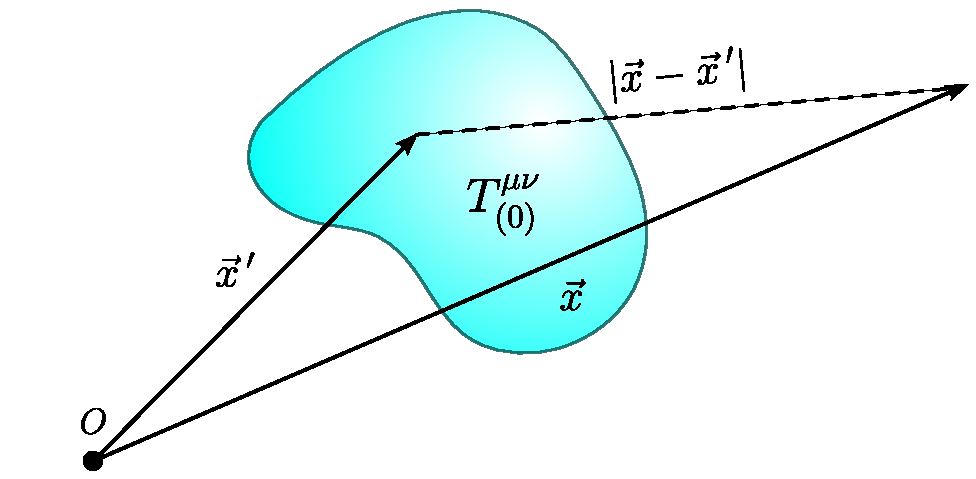
\includegraphics[width=\linewidth]{Emision-GW-1}
        \caption{Distribución de energía-momentum.}
        \label{fig:emision-GW-1}
    \end{subfigure}\hskip 1em%
    \begin{subfigure}[t]{0.39\textwidth}
        \centering
        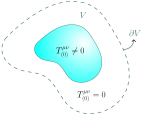
\includegraphics[width=\linewidth]{Emision-GW-2}
        \caption{Volumen que encierra la distribución de energía-momentum.}
        \label{fig:emision-GW-2}
    \end{subfigure}
\end{figure}

Por lo tanto, al comparar \eqref{eq:Emission-GW-3} y \eqref{eq:Emission-GW-4}, se obtiene que
\begin{equation}
\int_{V} T_{(0)}^{ij} d^3 x = \frac{1}{c} \frac{d}{dt} \int T_{(0)}^{i0} x^{j} d^3x.\label{eq:Emission-GW-5}
\end{equation}

Como $T^{ij}$ es simétrico, podemos escribir
\begin{align}
\int_{V} T_{(0)}^{ij} d^3 x &= \frac{1}{2} \int_{V} \left( T_{(0)}^{ij}  + T_{(0)}^{ji}\right) d^3 x \nonumber \\
&= \frac{1}{2c} \frac{d}{dt} \int_{V} \left( T_{(0)}^{i0} x^{j} + T_{(0)}^{j0} x^{i}\right) d^3x. \label{eq:Emission-GW-6}
\end{align}

Efectuamos ahora un análisis similar con la expresión $\int \partial_{k} (T_{(0)}^{0k} x^{i} x^{j}) d^3x $, que también es nula, pues, por el teorema de Gauss, se puede transformar en una integral de superficie en el borde de $V$ fuera de la región con fuentes. Entonces,
\begin{align}
0 &= \int_{V} \partial_{k} (T_{(0)}^{0k} x^{i} x^{j}) d^3x \nonumber \\
&= \int_{V} \partial_{k} (T_{(0)}^{0k}) x^{i} x^{j} d^3x + \int_{V}  T_{(0)}^{0k} \delta^{i}_{k} x^{j} d^3x + \int_{V}  T_{(0)}^{0k} x^{i}\delta^{j}_{k}  d^3x \nonumber \\
&= \int_{V} \partial_{k} (T_{(0)}^{0k}) x^{i} x^{j} d^3x + \int_{V} \left(T_{(0)}^{0i} x^{j} + T_{(0)}^{0j} x^{i} \right) d^3x.\label{eq:Emission-GW-7}
\end{align}

Usando \eqref{eq:Emission-GW-2}, cambiando el índice espacial $i$ por el temporal $0$,  la ecuación \eqref{eq:Emission-GW-7} nos queda

\begin{align}
0 &= - \int_{V} \partial_{0} (T_{(0)}^{00}) x^{i} x^{j} d^3x + \int_{V} \left(T_{(0)}^{0i} x^{j} + T_{(0)}^{0j} x^{i} \right) d^3x \nonumber \\
&= - \frac{1}{c} \frac{d}{dt} \int_{V} T_{(0)}^{00}x^{i}x^{j} d^3 x + \int_{V} \left(T_{(0)}^{0i} x^{j} + T_{(0)}^{0j} x^{i} \right) d^3x.
\end{align}

Por lo ranto,
\begin{equation}
\int_{V} \left(T_{(0)}^{0i} x^{j} + T_{(0)}^{0j} x^{i} \right) d^3x = \frac{1}{c} \frac{d}{dt} \int_{V} T_{(0)}^{00}x^{i}x^{j} d^3 x.\label{eq:Emission-GW-8}
\end{equation}

De esta forma, usando \eqref{eq:Emission-GW-6} y \eqref{eq:Emission-GW-8} encontramos que
\begin{equation}
\int_{V} T_{(0)}^{ij} d^3x = \frac{1}{2c^2} \frac{d^2}{dt^2} \int_{V} T_{(0)}^{00} x^{i} x^{j} d^3x. \label{eq:Emission-GW-9}
\end{equation}

Reemplazando \eqref{eq:Emission-GW-9} en \eqref{eq:metric-pert-rad}, podemos escribir que
\begin{equation}
\bar{h}^{ij}_{\text{rad}}(\vec{x},t) = - \frac{2G}{c^4} \frac{1}{r} \frac{d^2}{dt^2} \left[ \frac{1}{c^2} \int_{V} T_{(0)}^{00}(x') x^{'i} x^{'j} d^3x'\right]_{\text{ret}}.
\end{equation}

Como $T_{(0)}^{00}/c^2 = \rho(\vec{x},t)$ es la densidad de masa de la fuente (a primer orden), se acostumbra a escribir 
\begin{shaded}
\begin{equation}
\bar{h}^{ij}_{\text{rad}}(\vec{x},t) = - \frac{2G}{c^4} \frac{1}{r} \left[\ddot{M}^{ij} \right]_{\text{ret}}, \label{eq:metric-pert-rad}
\end{equation}
\end{shaded}
\noindent donde
\begin{equation}
M^{ij}(t) := \int_{V} \rho(\vec{x},t) x^{i} x^{j} d^3x,
\end{equation}
es el tensor momento de inercia (con traza) de la fuente. 

\subsection{Ejemplo:}

Consideremos dos cuerpos, cada uno de masa $M$, con una separación $2R$ que rotan en un movimiento no-relativista con velocidad angular $\omega$ en torno al centro de masa del sistema. Si inicialmente los cuerpos se encontraban en $\vec{x}_1(t = 0) = (0,0,0)$ y $\vec{x}_2(t = 0) = (-R,0,0)$, las posiciones de las masas están dada por
\begin{align}
\vec{x}_1 &= (x_1, y_1, z_1) = (R\cos(\omega t), R\sin(\omega t),0), \\
\vec{x}_2 &= (x_2, y_2, z_2) = (R\cos(\omega t + \pi), R\sin(\omega t + \pi),0) = - \vec{x}_1.
\end{align} 


\begin{figure}
     \centering
     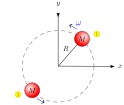
\includegraphics[scale = 0.58]{Ejemplo-Emision-GW}
     \caption{Sistema binario de dos masas $M$ rotando en un círculo de radio $R$ y rapidez angular $\omega$.}
     \label{fig:Example-emision-GW}
\end{figure}

En este caso, donde la distribución de masa no es continua, tenemos que
\begin{equation}
\int \rho x^{i} x^{j} dV \rightarrow \sum m x^{i} x^{j}.
\end{equation}

Las únicas componentes no nulas del momento cuadrupolar gravitacional son:
\begingroup
\allowdisplaybreaks
\begin{align}
M^{xx} &= m_1 x_1x_1 + m_2 x_2 x_2 \nonumber \\
&= M R^2 \cos^2(\omega t) + M R^2 \cos^2(\omega t) \nonumber \\
&= 2 M R^2 \cos^2(\omega t) \nonumber \\
&= M R^2 \left[ 1 + \cos(2\omega t)\right], \\
M^{xy} &= m_1 x_1y_1 + m_2 x_2 y_2 \nonumber \\
&= 2M R^2 \sin(\omega t) \cos(\omega t) \nonumber \\
&= MR^2 \sin(2\omega t), \\
M^{yy} &=  m_1 y_1y_1 + m_2 y_2 y_2 \nonumber \\
&= M R^2 \sin^2(\omega t) + M R^2 \sin^2(\omega t) \nonumber \\
&= 2M R^2 \sin^2(\omega t) \nonumber \\
&= MR^2 \left[1 - \cos(2\omega t) \right]. 
\end{align}
\endgroup

Pero, $M^{xz} = M^{yz} = M^{zz} = 0$, ya que el movimiento es en el plano $xy$.

Derivando con respecto al tiempo dos veces,
\begin{align}
\ddot{M}^{xx} &= - 4 MR^2 \omega^2\cos(2\omega t), \\
\ddot{M}^{xy} &= - 4 MR^2 \omega^2\sin(2\omega t), \\
\ddot{M}^{yy} &=  4 MR^2 \omega^2\cos(2\omega t).
\end{align}

En representación matricial, 
\begin{shaded}
\begin{equation}
\ddot{M}^{ij} = -4MR^2\omega^2 \begin{pmatrix}
\cos(2\omega t) & \sin(2\omega t) & 0 \\
\sin(2\omega t) & -\cos(2\omega t) & 0 \\
0 & 0 & 0
\end{pmatrix}
\end{equation}.
\end{shaded}

Con esto, \eqref{eq:metric-pert-rad} implica que\\
\begingroup
\allowdisplaybreaks
\begin{align}
\bar{h}_{\text{rad}}^{ij}(\vec{x},t) &= - \frac{2G}{c^4} \frac{1}{r}  \left[-4MR^2\omega^2\begin{pmatrix}
\cos(2\omega t_{\text{ret}}) & \sin(2\omega t_{\text{ret}}) & 0 \\
\sin(2\omega t_{\text{ret}}) & -\cos(2\omega t_{\text{ret}}) & 0 \\
0 & 0 & 0
\end{pmatrix} \right]_{t_{\text{ret}} = t - r/c} \nonumber \\
&= \frac{8GMR^2 \omega^2}{c^4 r} \begin{pmatrix}
\cos[2\omega (t - r/c)] & \sin[2\omega (t - r/c)] & 0 \\
\sin[2\omega (t - r/c)] & -\cos[2\omega (t - r/c)] & 0 \\
0 & 0 & 0
\end{pmatrix} \nonumber \\
&= \frac{8GMR^2 \omega^2}{c^4 r} \left[ \begin{pmatrix}
1 & 0 & 0 \\
0 & -1 & 0 \\
0 & 0 & 0
\end{pmatrix} \cos[2\omega(t - r/c)] + \begin{pmatrix}
0 & 1 & 0 \\
1 & 0 & 0 \\
0 & 0 & 0
\end{pmatrix} \sin[2\omega(t - r/c)]\right] \nonumber \\
&= \frac{8GMR^2 \omega^2}{c^4 r} \left[ \begin{pmatrix}
1 & 0 & 0 \\
0 & -1 & 0 \\
0 & 0 & 0
\end{pmatrix} \cos[2\omega(t - r/c)] + \begin{pmatrix}
0 & 1 & 0 \\
1 & 0 & 0 \\
0 & 0 & 0
\end{pmatrix} \cos[2\omega(t - r/c) - \pi/2]\right] \nonumber \\
&= \frac{8GMR^2 \omega^2}{c^4 r} \Re \left[ \begin{pmatrix}
1 & 0 & 0 \\
0 & -1 & 0 \\
0 & 0 & 0
\end{pmatrix} e^{i[2\omega(t - \frac{r}{c})]} + \begin{pmatrix}
0 & 1 & 0 \\
1 & 0 & 0 \\
0 & 0 & 0
\end{pmatrix} e^{i[2\omega(t - \frac{r}{c})- \frac{\pi}{2}] } \right] .
\end{align}
\endgroup

Vemos de aquí que un observador ubicado en un punto sobre el eje $z$ detectará una onda gravitacional de frecuencia angular $2\omega$, que satisface automáticamente el gauge TT, y que es una combinación lineal de las polarizaciones $+$ y $\times$, con una diferencia de fase de $\pi/2$. Este estado es análogo al de una onda electromagnética con polarización circular.

El orden de magnitud de la amplitud de la onda es dada por
\begin{equation}
h \simeq \frac{8GMR^2 \omega^2}{c^4 r} = 8 \left( \frac{GM}{c^2}\right) \left( \frac{1}{r}\right) \left( \frac{\omega R}{c}\right)^2 = 8 \left(\frac{m}{r} \right) \left( \frac{v}{c}\right)^2,
\end{equation}
donde $v = \omega R$ es la rapidez de un objeto en un movimiento circular de radio $R$ con frecuencia angular $\omega$.

Por ejemplo, el pulsar binario PSR 1913+16 consta de dos estrellas de neutrones de masa $M \approx 1.4 M_{\odot}$, con periodo orbital $T \approx 8 \,\text{h} \approx 3 \times 10^{4} \, \text{s}$, velocidades orbitales $v \simeq 10^2 \,\text{km/s}$, a una distancia $r \approx 2 \times 10^{4} \,\text{ly} \approx 10^{20}\, \text{m}$. 

Para calcular $h$, se necesitan los siguientes datos: \footnote{Datos sacados de \url{
https://physics.nist.gov/cuu/Constants/}}
\begin{align}
G &= 6.67430 \times 10^{-11} \,\left[ \frac{m^3}{kg \,s^2} \right], \quad  c =  299 792 458 \,\left[ \frac{m}{s}\right], \quad  M_{\odot} = 1.988 \times 10^{30} \,[kg]. 
\end{align}

Así, obtenemos que
\begin{align}
m &= \frac{(6.67430 \times 10^{-11}) \cdot 1.4 \cdot (1.988 \times 10^{30}) }{(299 792 458)^2} \,[km]\approx 2.067 \,[km], \\
\frac{v}{c} &= \frac{10^{5}}{299 792 458} \approx 3 \times 10^{-4}.
\end{align}

Por lo tanto, la amplitud de la onda gravitacional es
\begin{equation}
h \simeq 8 \cdot \left( \frac{2.067 \times 10^{3}}{10^{20}}\right) (3 \times 10^{-4})^2 \approx 1.4 \times 10^{-23},
\end{equation}
a una frecuencia del orden de $1/T \sim 10^{-4} \,[Hz]$.
\end{document}

